\chapter{Odor discrimination task in mice}
\label{chap:MaxData}
%\section{Introduction}
We present an application of the cell-assembly algorithm, at level of pairs, on electrophysiological data from mice.
Dual side in-vivo recordings of electophysiological activity from Ventral Striatum, including Pallidum, (VS) and Ventral Tegmental Area (VTA), allowed us to study directionality between the two regions.
The novel statistical approach presented treats the temporal scale and precision of coherent activity patterns as free parameters, to be determined from the data, thus, instead to make assumption, we deduced from data temporal scales and precision involved in assemblies pairs with units either from both regions or from only one of the two regions, shedding light on VS-VTA interaction temporal structure and directionality.
Taking advantage of well defined neuron typologies classifications both in VS and VTA, we further investigated the specific cell-type composition of the assemblies exhibiting directionality. 
%According to their response properties, neurons in VTA are classified in Type I (dopaminergic), Type II(GABAergic) and Type III; according to their electrophysiological properties, neurons in VS are di-vided in medium spiny neurons (MSN), cholinergic interneurons (CIN), and fast spiking interneurons(FSI), the latter are mostly pallidal units.
\section{Description of experiment and data set}
The task was a go-no go reversal odor discrimination task. Two odors were presented to the mouse, one rewarded (CS+) with reward probability 0.9, the other one not rewarded (CS-). Learning the task consisted in licking at least twice when CS+ was presented (hit trials) and not licking during or after the CS- presentation (correct rejection trials). Once the performance criterion was reached, contingencies were switched. Lick window was open for an interval ranging from 1500 $ms$ to 2000 $ms$ for different sessions after a delay from 500 $ms$ to 1500 $ms$. Only licks happening in the lick window interval were counted as valid to get the reward.
\section{Single cells analysis}
\section{Preliminary cell assemblies results}
Preliminary cell assemblies analysis were aimed to understand the size of the concentration of the shared pairs, namely how many units are involved in pairs and, among those, how the units typologies are distributed.
{\color{red} Include figure pie charts for all reversal paradigma}
\section{Time scales, directionality}
Applying the cell-assembly algorithm we were able to detect synchronous ($lag=0$) and asynchronous ($lag\neq 0$) cell assemblies at arbitrary time scale ($\Delta$). Time scales distribution results to be different for intra- regional assembly pairs (pairs with units from VS or VTA) and inter-regional assemblies pairs (pairs with units from both VS and VTA). It's important to point out that, in case of inter-regional pairs, the lag distribution it's a instruments to measure directionality between two regions, indicating which unit fires first leading the activation pattern activity and which one consequently follows. In our case $lag >0$ means VS precedes in activity VTA, and $lag <0$ the opposite, $lag=0$ means that the two units are  simultaneous in activation at the precision of the time scale at which are detected.
We start our analysis from time scales distribution involved in detection pairs.
\begin{figure}[H]
\centering
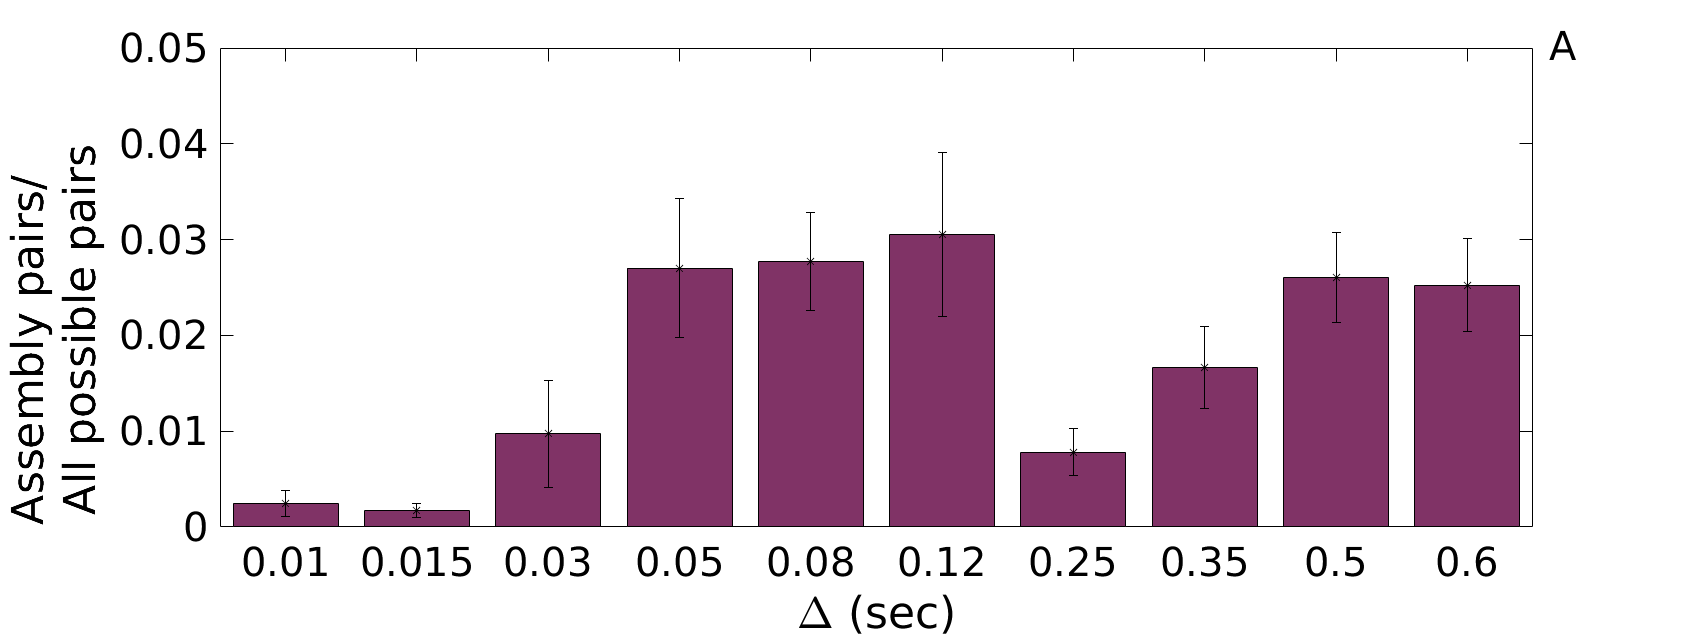
\includegraphics[scale=0.2]{figures/VS_VTA_SLet.png}
%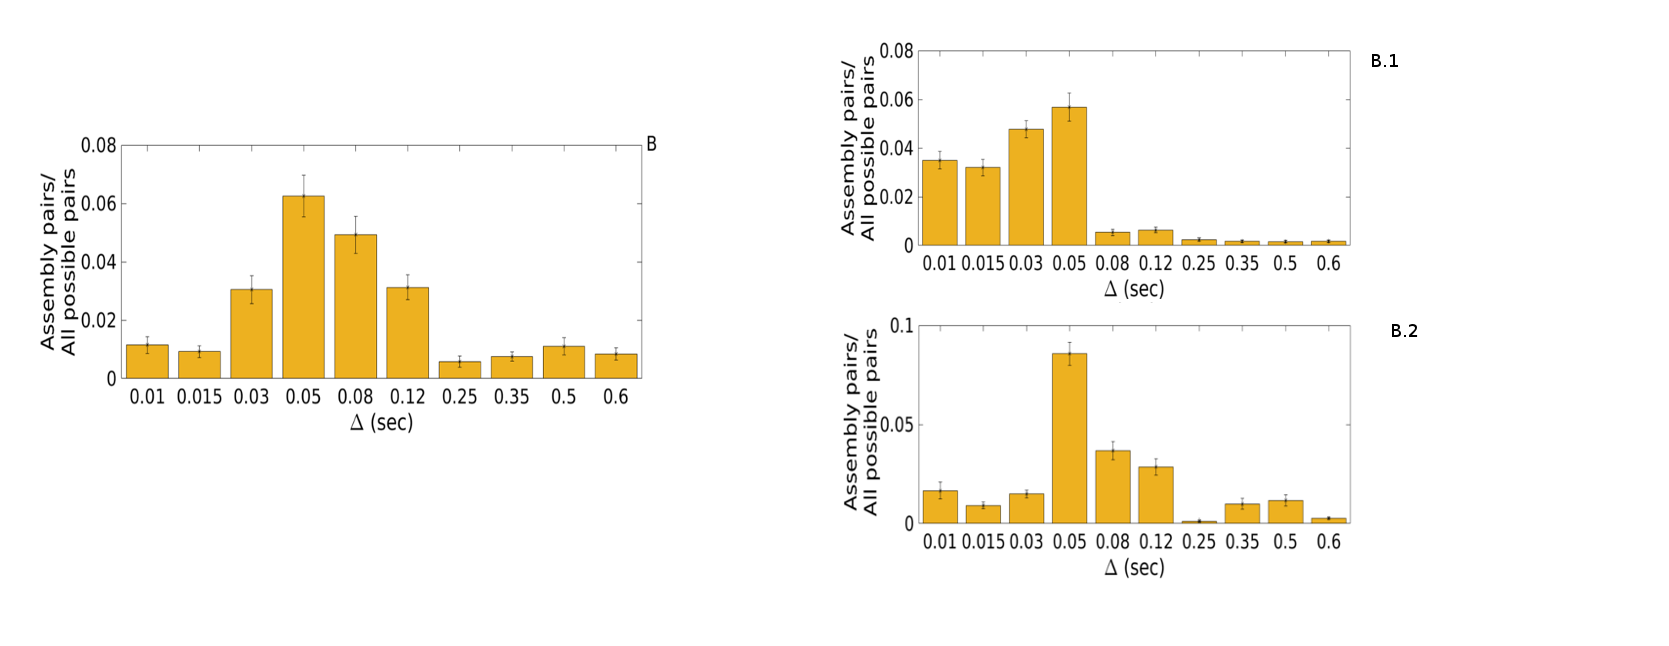
\includegraphics[scale=0.4]{figures/VS_VS_SLet1.png}
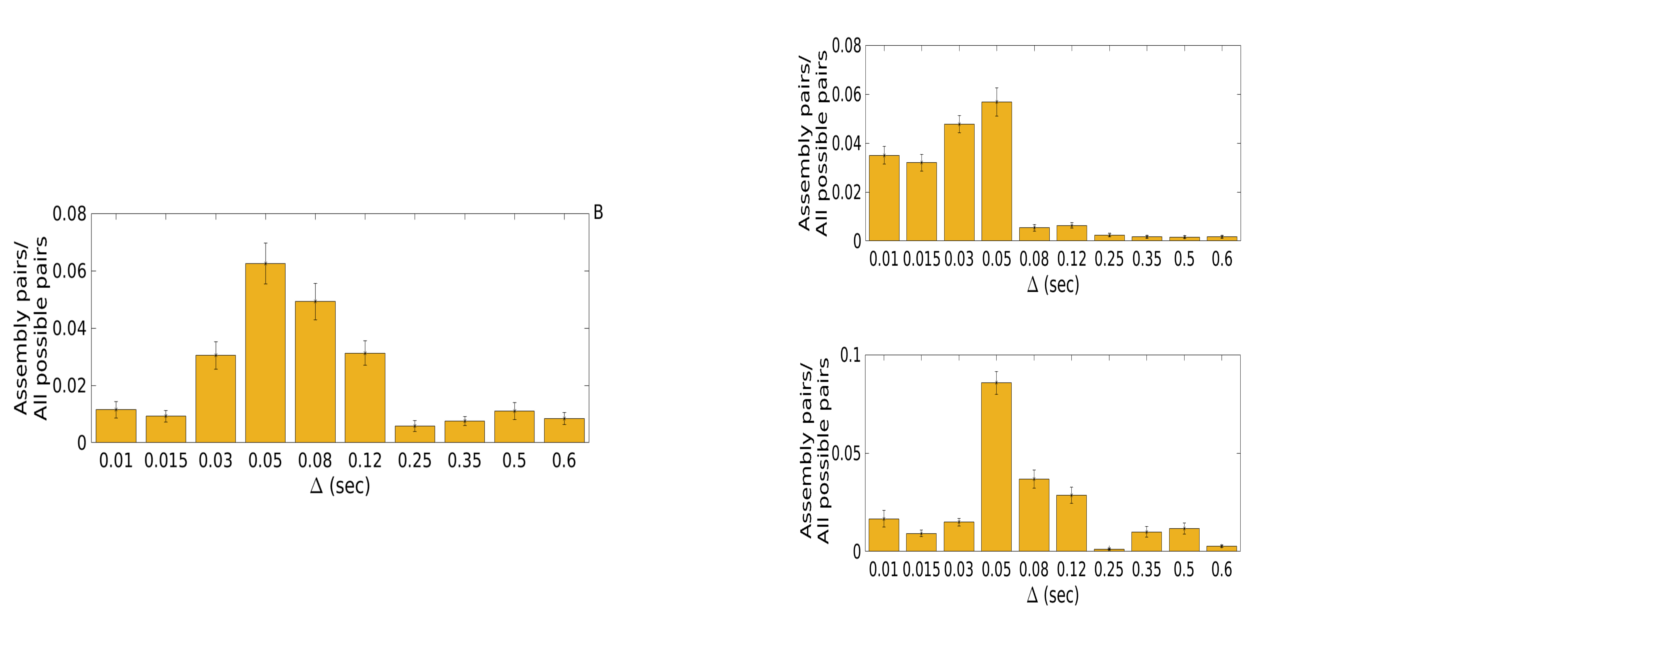
\includegraphics[scale=0.4]{figures/AllBinVSVS.png}
%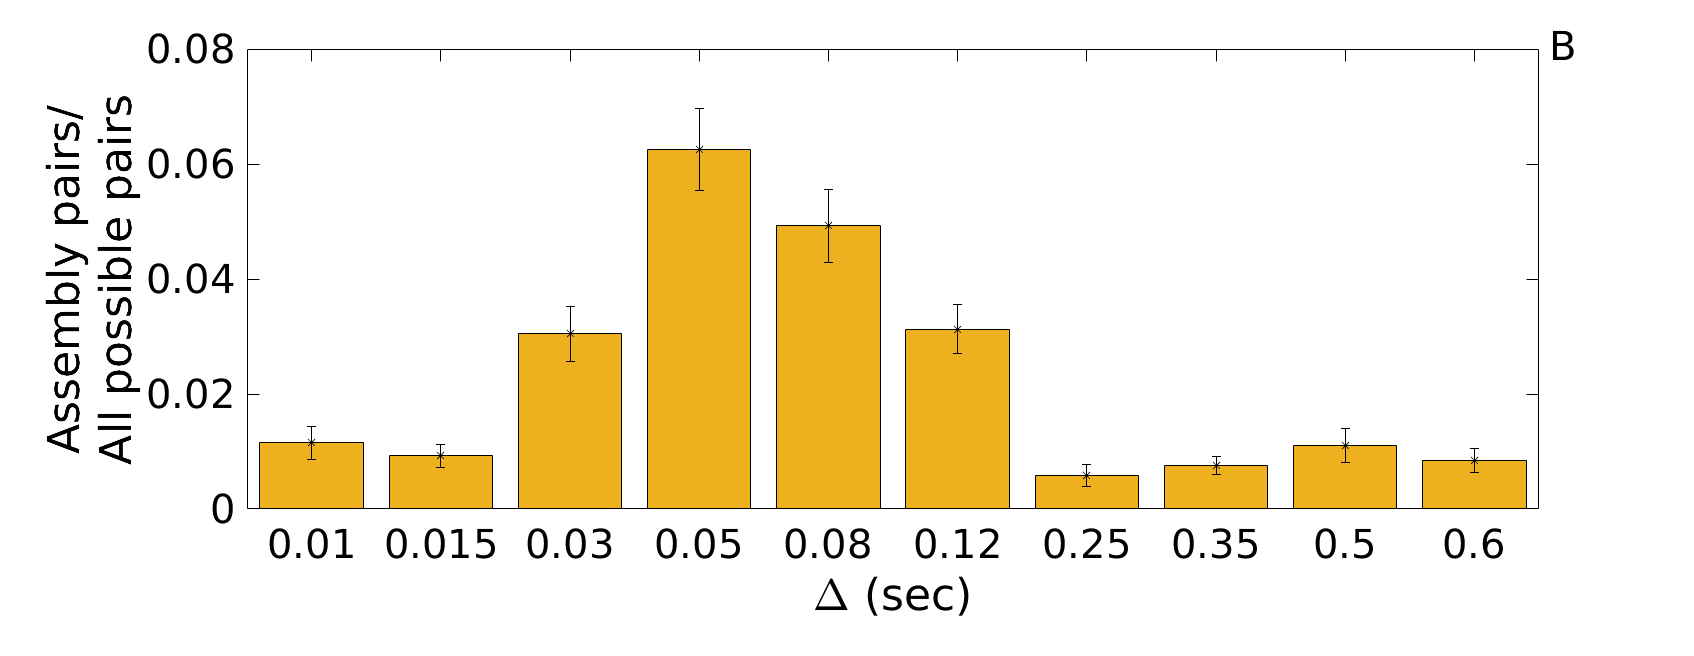
\includegraphics[scale=0.2]{figures/VS_VS_SLet.png}
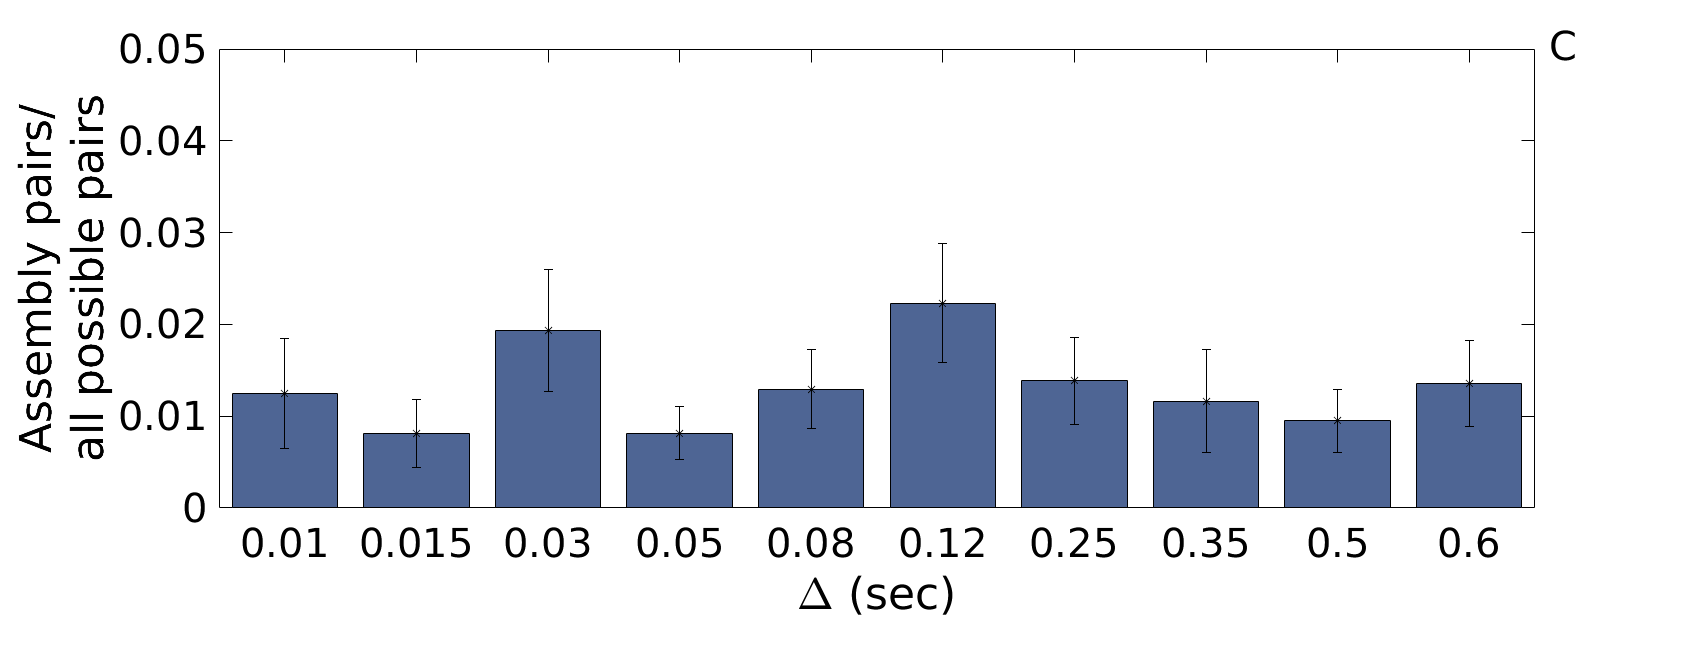
\includegraphics[scale=0.2]{figures/VTA_VTA_SLet.png}

\caption{{\color{red}Important!! Re do the figures with GIMPS include text with title} Bin distribution for intra-regional and inter-regional pairs. A) VS-VTA pairs show a bimodal distribution, meaning two temporal scale involved in inter-regional activtion patterns. B) VS-VS pairs bin distribution presents a peak at 50 $ms$, specifically in this region the pairs MSN-FSI high show an highly peaked distribution, almost centered at the peak of 50 $ms$, plot (B.2), while in MSN-FSI low distribution, albeit the peak is still at 50 $ms$, is evident the predominance of very precise time scales, including bins from 10 $ms$ to 50 $ms$, with respect to the larger time scale plot (B.1).}
\label{fig:BinDistr}
\end{figure}
Clear differences in time scales distribution of pairs detected in VS, VTA and VS-VTA emerge in fig.(\ref{fig:BinDistr}). Inter-regional pairs (VS-VTA) have a time scales distribution with a peak around 80 $ms$ while. Two time scales clearly emerge, the first, preciser, ranged from 10 $ms$ to 250 $ms$, and the latter, broader, peaked at 1.6 $s$. Intra-regional VTA-VTA pairs instead don't present any peak in time scales distribution. Intra-regional VS-VS bin size distribution is peaked around 50 $ms$. In VS we noticed differences between MSN and high-firing-rate FSI pairs and MSN and low-firing-rate FSI bin size distributions: specifically the firsts show higher temporal precision than the latter. {\color{red}{Include Figure of MSN-FSI and caption of bin size distribution}}.
Directionality between VS and VTA was a point of particular interest for our study. We studied separately lag distribution of VS-VTA pairs detected in the preciser and broader temporal scales, as highlighted from bin sizes distribution. Preciser VS-VTA pairs show slight directionality in the direction VS (fig. \ref{fig:LagInSecAll}). A zoom in preciser VS-VTA pairs reveals the directionality being mainly carried by MSN-Type I pairs.
\begin{figure}[H]
\centering
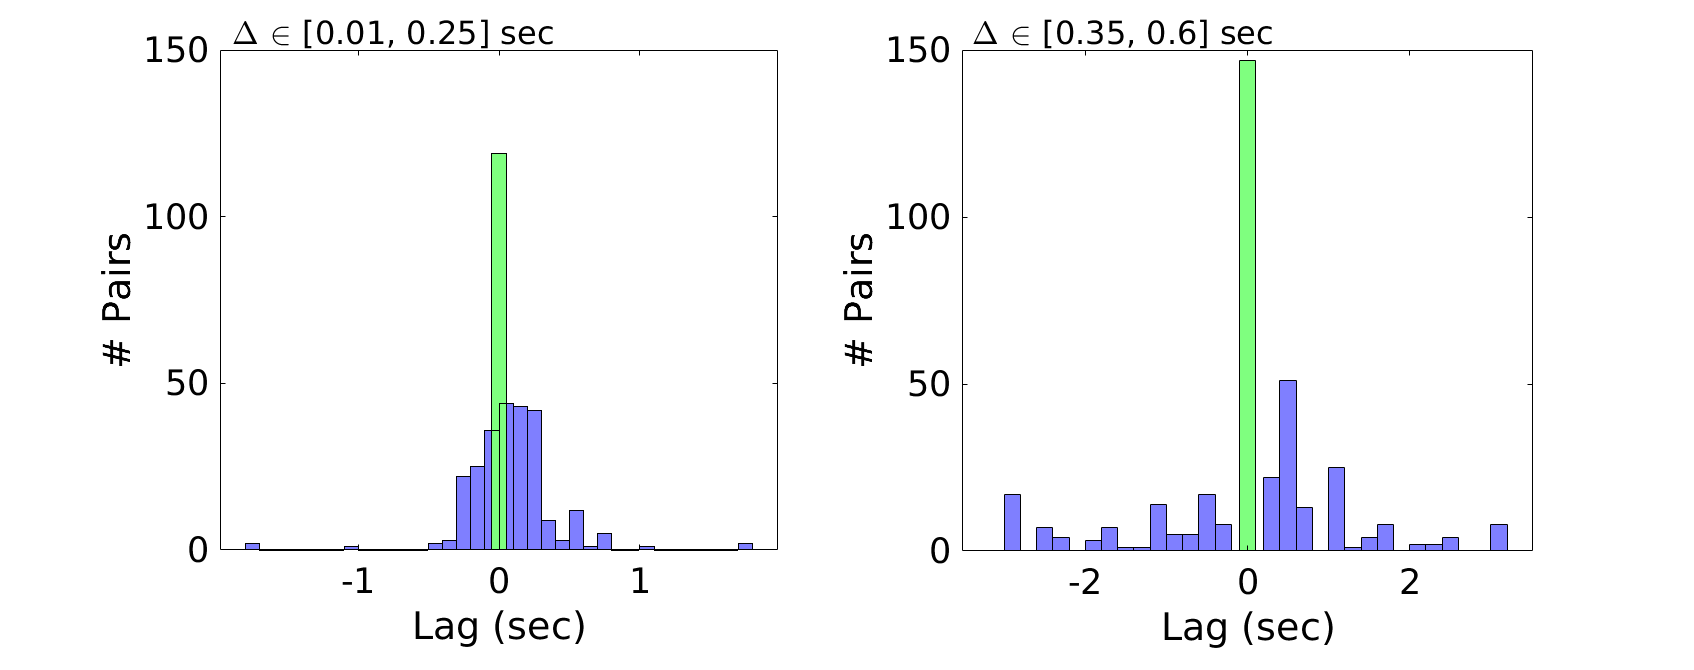
\includegraphics[scale=0.3]{figures/LagGeneralInSec.png}
\caption{Lag distribution for VS-VTA pairs in seconds. In green the synchronous pairs. On the left, lag distribution for pairs detected in preciser time scales. Slight distribution asymmetry indicates directionality in the direction of $lag > 0$, meaning a predominance of pairs in which VS leads VTA. On the right, the lag distribution for pairs detected in the broader time scale.}
\label{fig:LagInSecAll}
\end{figure}

\begin{figure}[H]
\centering
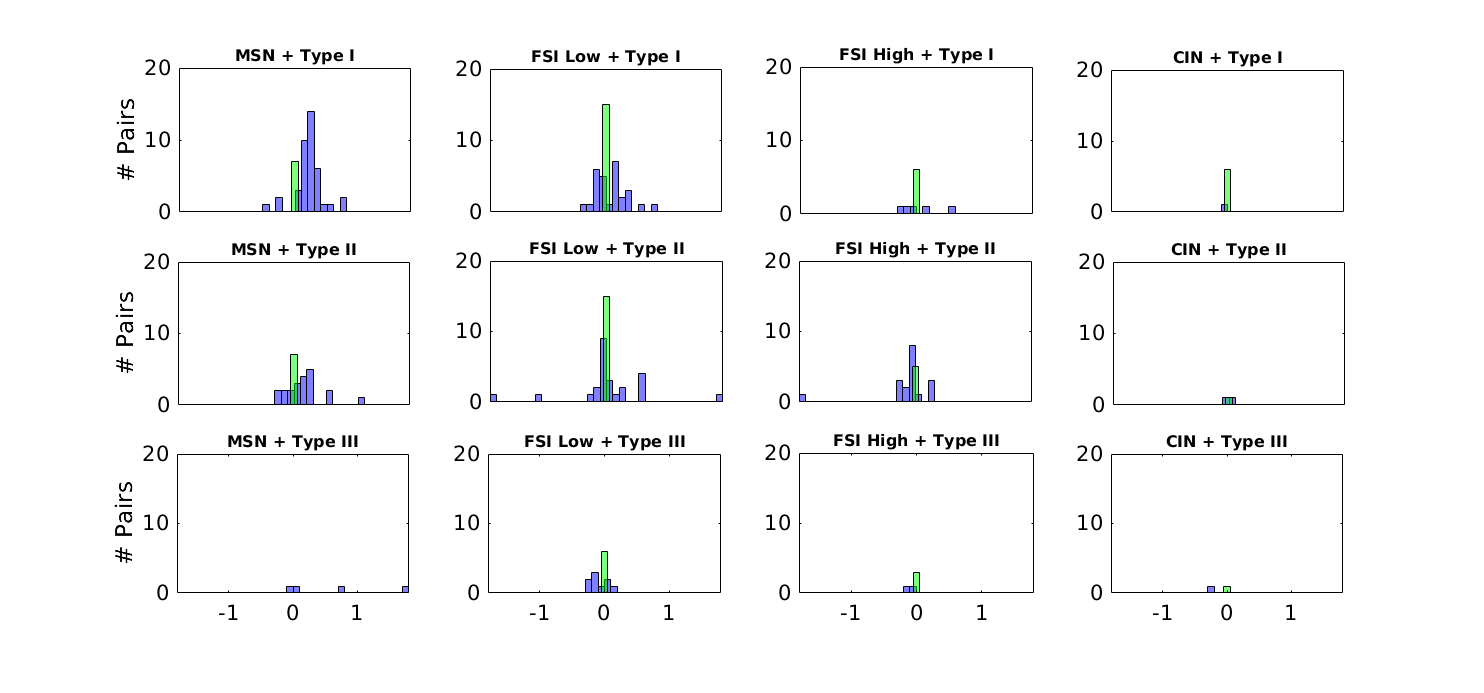
\includegraphics[scale=0.4]{figures/Type_oriz.png}
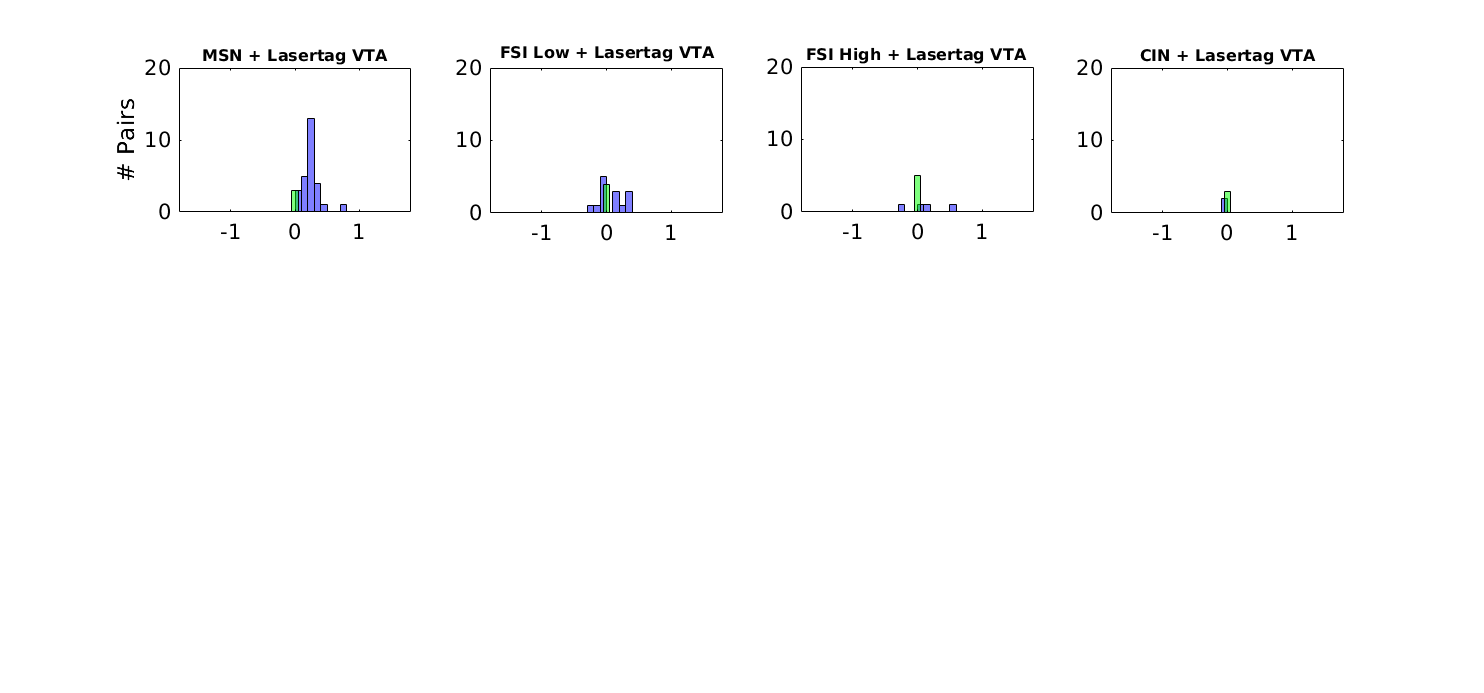
\includegraphics[scale=0.4]{figures/OnlyLaserOriz.png}
\caption{blabla}
\label{fig:LagInSecAll}
\end{figure}



%\section{Discussion}
%\section{Combination of single neuron and assemblies analysis}
%\subsection{Directionality using classification}
\subsection{Significant task related response for typology}
The assemblies were pruned according their significant task related activity, that was tested with Friedman's test and a non parametric version of the repeated measures Anova. We preferred to use non-parametric tests to be free from the assumption of gaussianity of the observations. Results of the two tests were consistent each other. The two relevant events of the task were the odor onset and the reward delivery, then we choose whether the assemblies showed a significant activity in three windows: Post-Stimulus [0s, 0.5s], Pre-Reward [-0.5s, 0s], Post-Reward [0s, 05s], the baseline was chosen in the interval [-0.8s, -0.3s] from the odor onset. Post-hoc analysis were performed using the Bonferroni's criterion {\color{red}check whether the criterion was Bonferroni of some other}
\section{Conclusion}
